\section{Desarrollo}

Cuando empezamos a diseñar el DER nos encontramos con varias dudas sobre algunas entidades y alguna de las
relaciones entre ellas. Luego de hacer las consultas con nuestro Tutor tuvimos que realizar algunos cambios. A continuaci\'on describiremos los cambios más importantes.

\subsection{Entidad Modalidad}

Entre los cambios más importantes, pueden destacarse aquellos relacionados con la exentidad \textbf{Modalidad}, que por enunciado, solo puede ser de 5 valores posibles y dependiendo del tipo de modo, esta posee distintos atributos. Lo primero que se nos ocurrio fue tenerla como entidad padre y luego como entidades hijas (disjuntas) a cada tipo de modalidad(forma, salto, etc).
Pero eso luego nos tra\'ia complicaciones para definir las relaciones entre Competencia y Modalidad, dado que había que poner muchas restricciones para que el modelo sea consistente con la especificación. 
Por ejemplo, si tuviesemos que registrar una competencia con una modalidad del tipo ''Forma", una de las restricciones hubiese sido: una competencia debe estar relacionada con uno de los tipos de modalidad. También que solo está relacionado con el Tipo ''Forma'' y no pude estar relacionado con otro tipo. 
Y también había que aclarar que una competencia podría no estar en la modalidad ''Forma". \\

Luego al consultarlo con el Tutor decidimos que no tenía tanta relevacia separar esa información en tantas entidades, si no que podr\'iamos almacenar toda esa información en una sola entidad. Agregando como restricciones que si la entidad era de detenerminado modo, entonces tenía que tener valores no nulos los atributos correspondientes a ese modo. \\

\subsection{Entidad Competencia}


Al principio pensamos esta entidad como una jerarqu\'ia, Competencia como entidad padre y Single y Team como entidades hijas. La entidad Single ser\'ia para las competencias entre competidores, y la entidad Team ser\'ia para las competencias entre equipos. Necesitabamos hacer esto para poder diferenciar que competencias eran de modalidad "combate por equipos" dado que tenía atributos caracter\'sticos. Con esto teníamos cubierto esa diferencia pero al observar m\'as en detalle la existencia de las entidad hijas, vimos que estas no tenían atributos característicos con respecto a su identidad padre, y que en definitiva al pasarlas a la base de datos solo guardar\'ian los campos claves de los competidores/equipos y con un Id de competencia relacionado.\\

Para simplificar el modelo lo que hicimos fue eliminar estas entidades hijas y pasamos la relacion "participa" de Competidor a Competendia y lo mismo para equipo. También agregamos las restricciones de que una competencia esta relacionada a competidores o a equipos, no puede pasar ambas a la vez.

\begin{center}
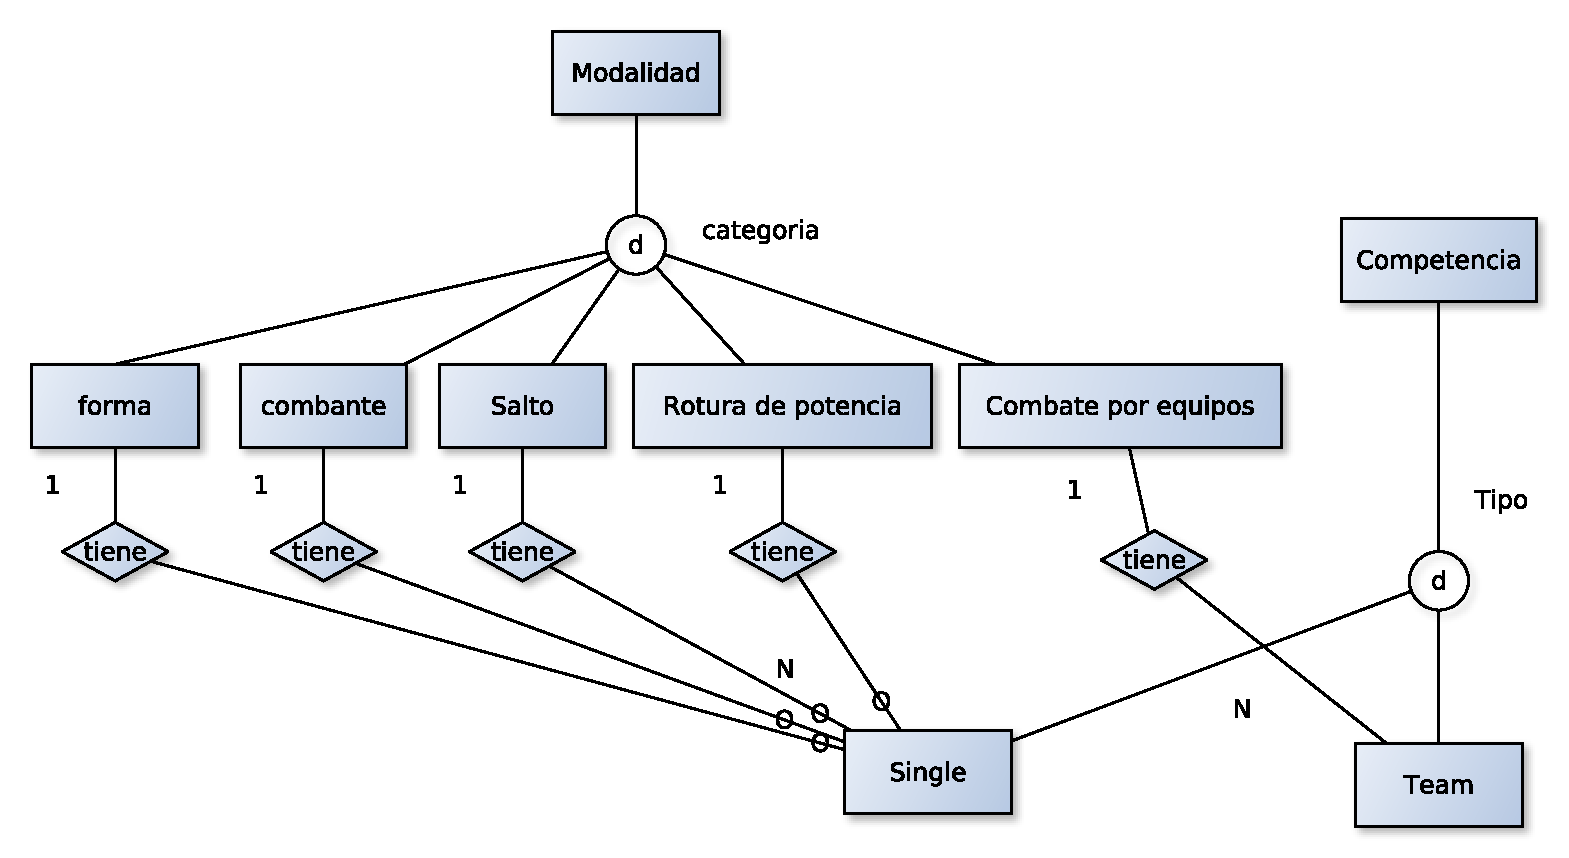
\includegraphics[width=12cm,keepaspectratio]{./imagenes/des1.pdf}\newline
\end{center}

\subsection{Entidad Match}

Dado que el enunciado ped\'ia obtener los ganadores de cada competencia: 1er, 2do y 3er lugar, pensamos en guardar la informaci\'on de los encuentros y obtener de ellos el resultado de los ganadores. La entidad Match guardar\'ia el id del competidor ganador y la fecha del encuentro. Para esto asumiamos que los dos \'ultimos encuentros ser\'ian las del 3er puesto y la final. Aca nos volvimos a encontrar con el problema de diferenciar los encuentros entre competidores y los de equipos, por lo cual teníamos que crear una jerarquía para obtener MatchIndividual y MatchGrupo. Y al igual que en el caso de la entidad Competencia ,estas entidades hijas carecían de atributos y s\'olo guardaban campos claves de otras entidades.

Luego de mostrarselo a nuestro benemérito Tutor, comprendimos que no había que guardar la información de los encuentros, y que s\'olo bastaba con que la competencia almacenara los Id de los competidores/equipos ganadores. Por ese decidimos eliminar la entidad Match y agregar los atributos necesarios a la Entidad Competencia para que guarde la informaci\'on de los ganadores.

\begin{center}
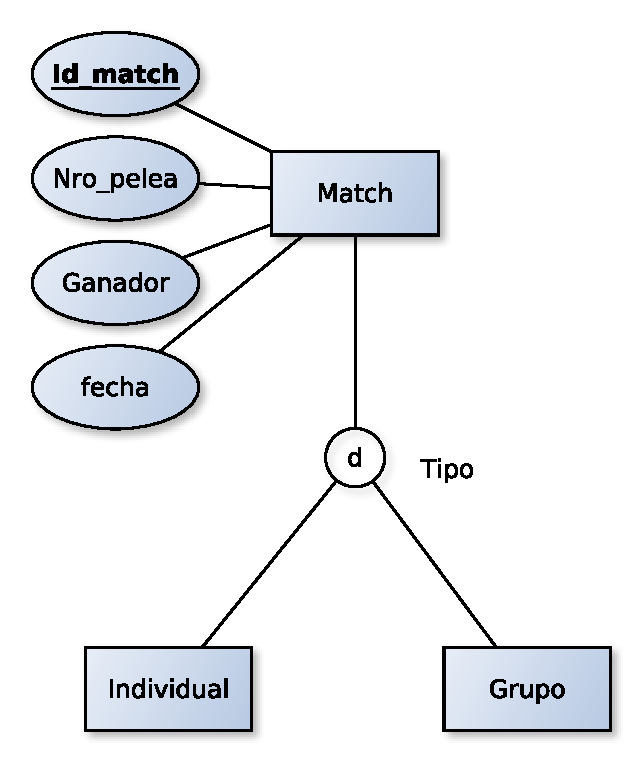
\includegraphics[width=6cm,keepaspectratio]{./imagenes/des2.pdf}\newline
\end{center}




